\chapter{Dataset}
In this chapter, we will describe the few-shot shell dataset we are introducing.

Many datasets exist for object detection. These can be split into two categories, general datasets and specialized datasets. General datasets are datasets that contain a wide variety of object classes, such as COCO \cite{COCO}, OpenImages \cite{OpenImages}, and ImageNet \cite{ImageNet}. Specialized datasets are datasets that contain a specific category of objects like Oxford Pets \cite{OxfordPets} and Gun Detection \cite{Gundetection}. The general datasets are often used to pre-train a model, while the specialized datasets are used to fine-tune the model to a specific task.

However, no such specialized object detection dataset exists for seashells. Getting a representative dataset of all or most types of shells that could be found in large quantities would be a very time-intensive task. As such we purposefully limit the size of the dataset, so that we can evaluate the performance on a small dataset. 

\section{Images}
The images were taken with a cellphone camera on the Belgian coast near Knokke-Heist. Each image has a size of 6144x8192px. The images are mostly sparse, with 1 to 3 shells per image. The dataset does however also contain a limited amount of denser images. An overview of the density can be found in Figure \ref{fig:annotations_per_img}. 

\begin{figure}[H]
    \centering
    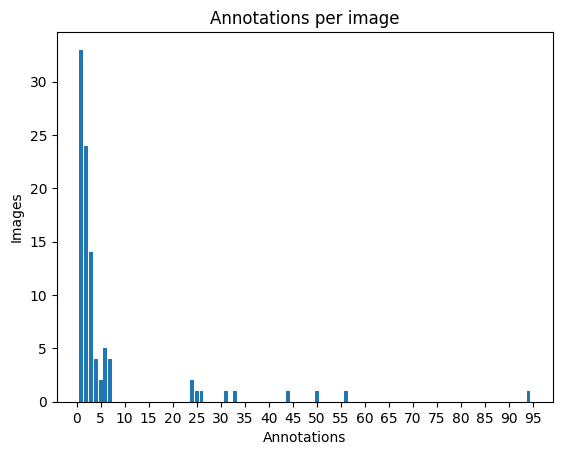
\includegraphics[width=0.8\textwidth]{chapter3/annotations_per_img.png}
    \caption{Overview of the annotations per image in the shell dataset.}
    \label{fig:annotations_per_img}
\end{figure}

\section{Annotations}
The images are annotated in Pascal VOC \cite{PASCALVOC} style. As such the annotations are saved in separate XML files, one for each image. In total 96 images are annotated with 614 annotations in total over 9 classes. As shown in Figure \ref{fig:annotations_per_class}% and Table \ref{tab:shell_annotations}
, the annotations are not evenly distributed over the classes. Some examples of the annotated images can be found in Figure \ref{tab:shell_examples}.


\begin{center}
    \begin{figure}[H]
        \makebox[\textwidth]{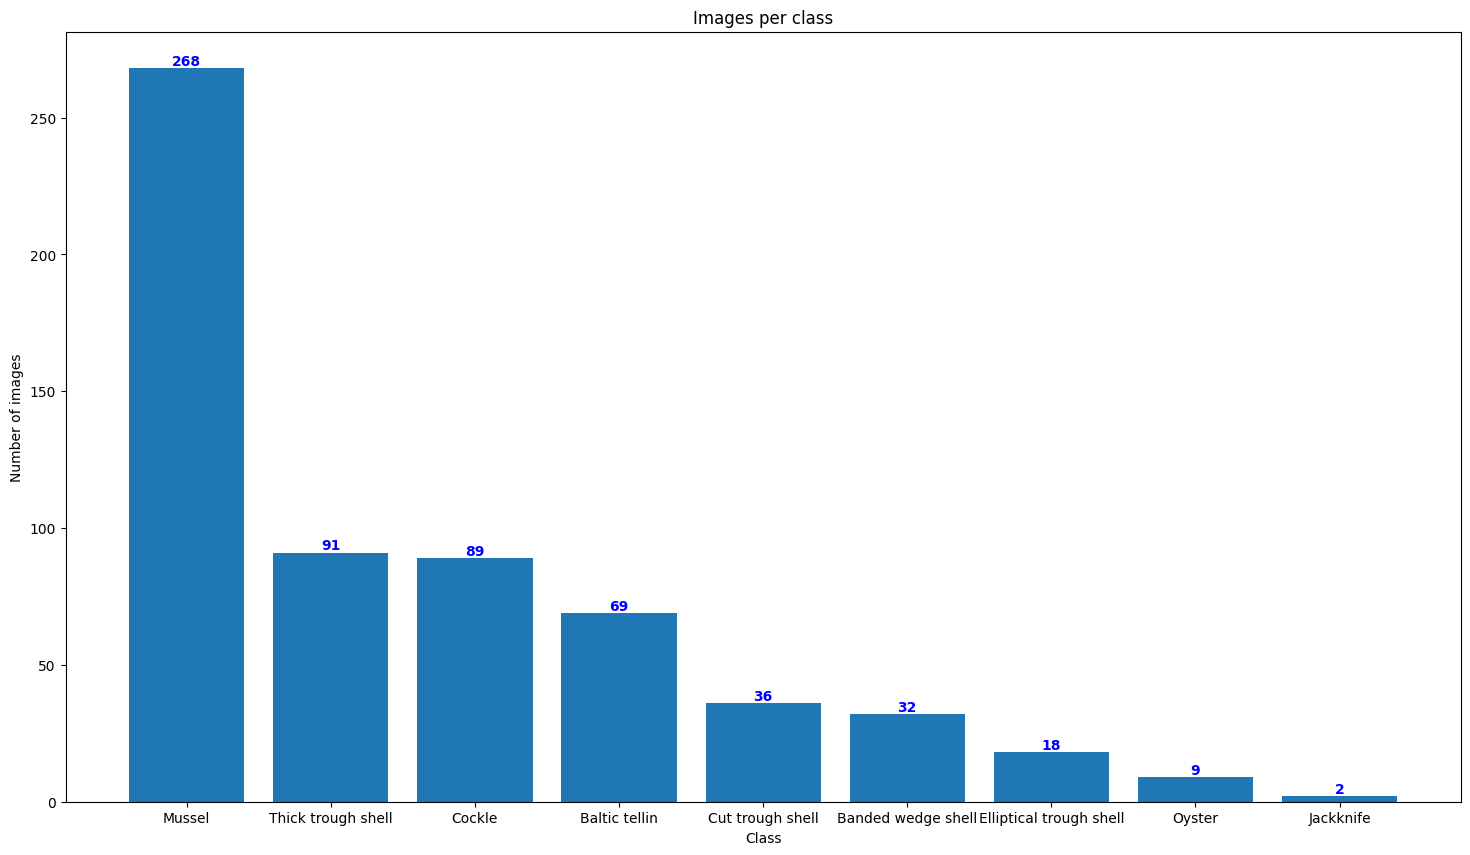
\includegraphics[width=0.9\paperwidth]{chapter3/annotations_per_class.png}}
        \caption{Overview of the annotations per class in the shell dataset.}
        \label{fig:annotations_per_class}
    \end{figure}
\end{center}



% \begin{table}[H]
%     \centering
%     \captionsetup{justification=centering}
%     \begin{tabular}{|l|l|}
%     \hline
%     \textbf{Shell type} & \textbf{Number of annotations} \\ \hline
%     Mussel              & 268                            \\ \hline
%     Thick trough shell  & 91                             \\ \hline
%     Cockle              & 89                             \\ \hline
%     Baltic tellin       & 69                             \\ \hline
%     Cut trough shell    & 36                             \\ \hline
%     Banded wedge shell  & 32                             \\ \hline
%     Elliptical trough shell & 18                         \\ \hline
%     Oyster              & 9                              \\ \hline
%     Jackknife clam      & 2                              \\ \hline
%     \end{tabular}
%     \caption{Overview of the annotations per class in the shell dataset.}
%     \label{tab:shell_annotations}
% \end{table}


\section{Limitations}
The dataset is limited in a few ways. In this section, we will discuss these limitations and their impact on our work.

\subsection*{Number of classes and size}

At the last shell-counting day a total of 51 types of shells were found in Belgium, with 66 types of shells being found when looking at all participating countries (Belgium, France, The Netherlands). However, only 8 types of shells are present in the dataset. This is due to the limited variety of shells that were found on the day the dataset was collected. Some shells are more difficult to find or are more rare than others, thus it would be difficult to collect a large number of images of these shells even if more images were collected. Realistically we would either have to put in a lot more time and effort to include sufficient shells of every type or find an alternative that uses less data to process our images. The practical results of our work will be limited to the shells that are present in the dataset, but still give a good indication as to what we can expect from it when applied to other shells.

The dataset consists of only 96 annotated images. This is an extremely small dataset, especially for object detection. Though it would be possible to collect and annotate more images, this would be a time-consuming task. Furthermore, the dataset is large enough to indicate the performance of the model as mentioned above.

\subsection*{Diversity}

The dataset is also limited in diversity, as all images were taken on the same day, at the same location, and with the same camera. This means that the dataset is not representative of the full range of conditions that the model would have to work in.


\begin{figure}[H]
    \centering
    \captionsetup{justification=centering}
    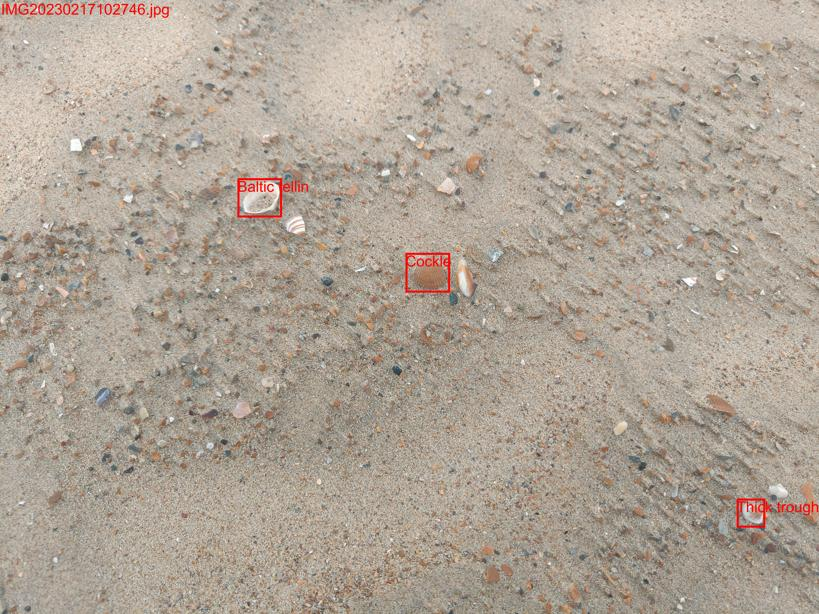
\includegraphics[width=0.3\textwidth]{chapter3/shell_examples/1.jpg} 
    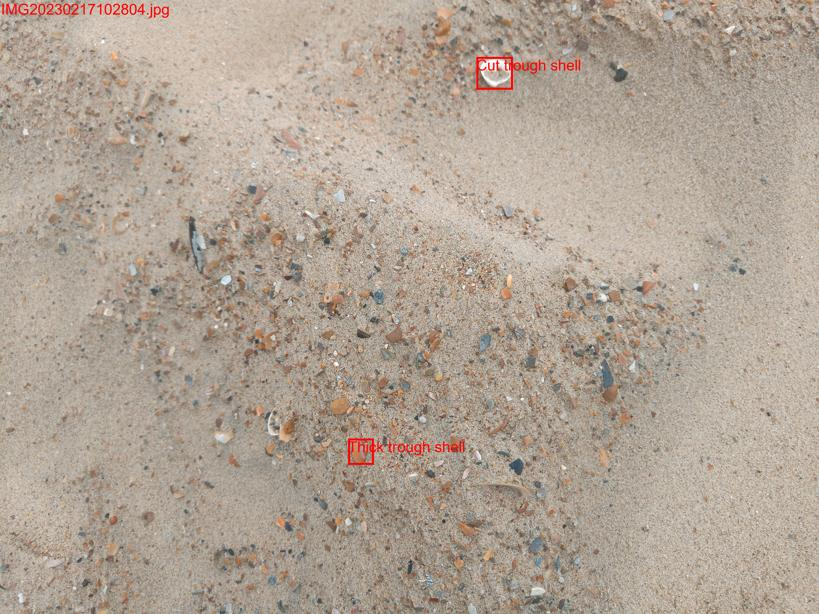
\includegraphics[width=0.3\textwidth]{chapter3/shell_examples/2.jpg} 
    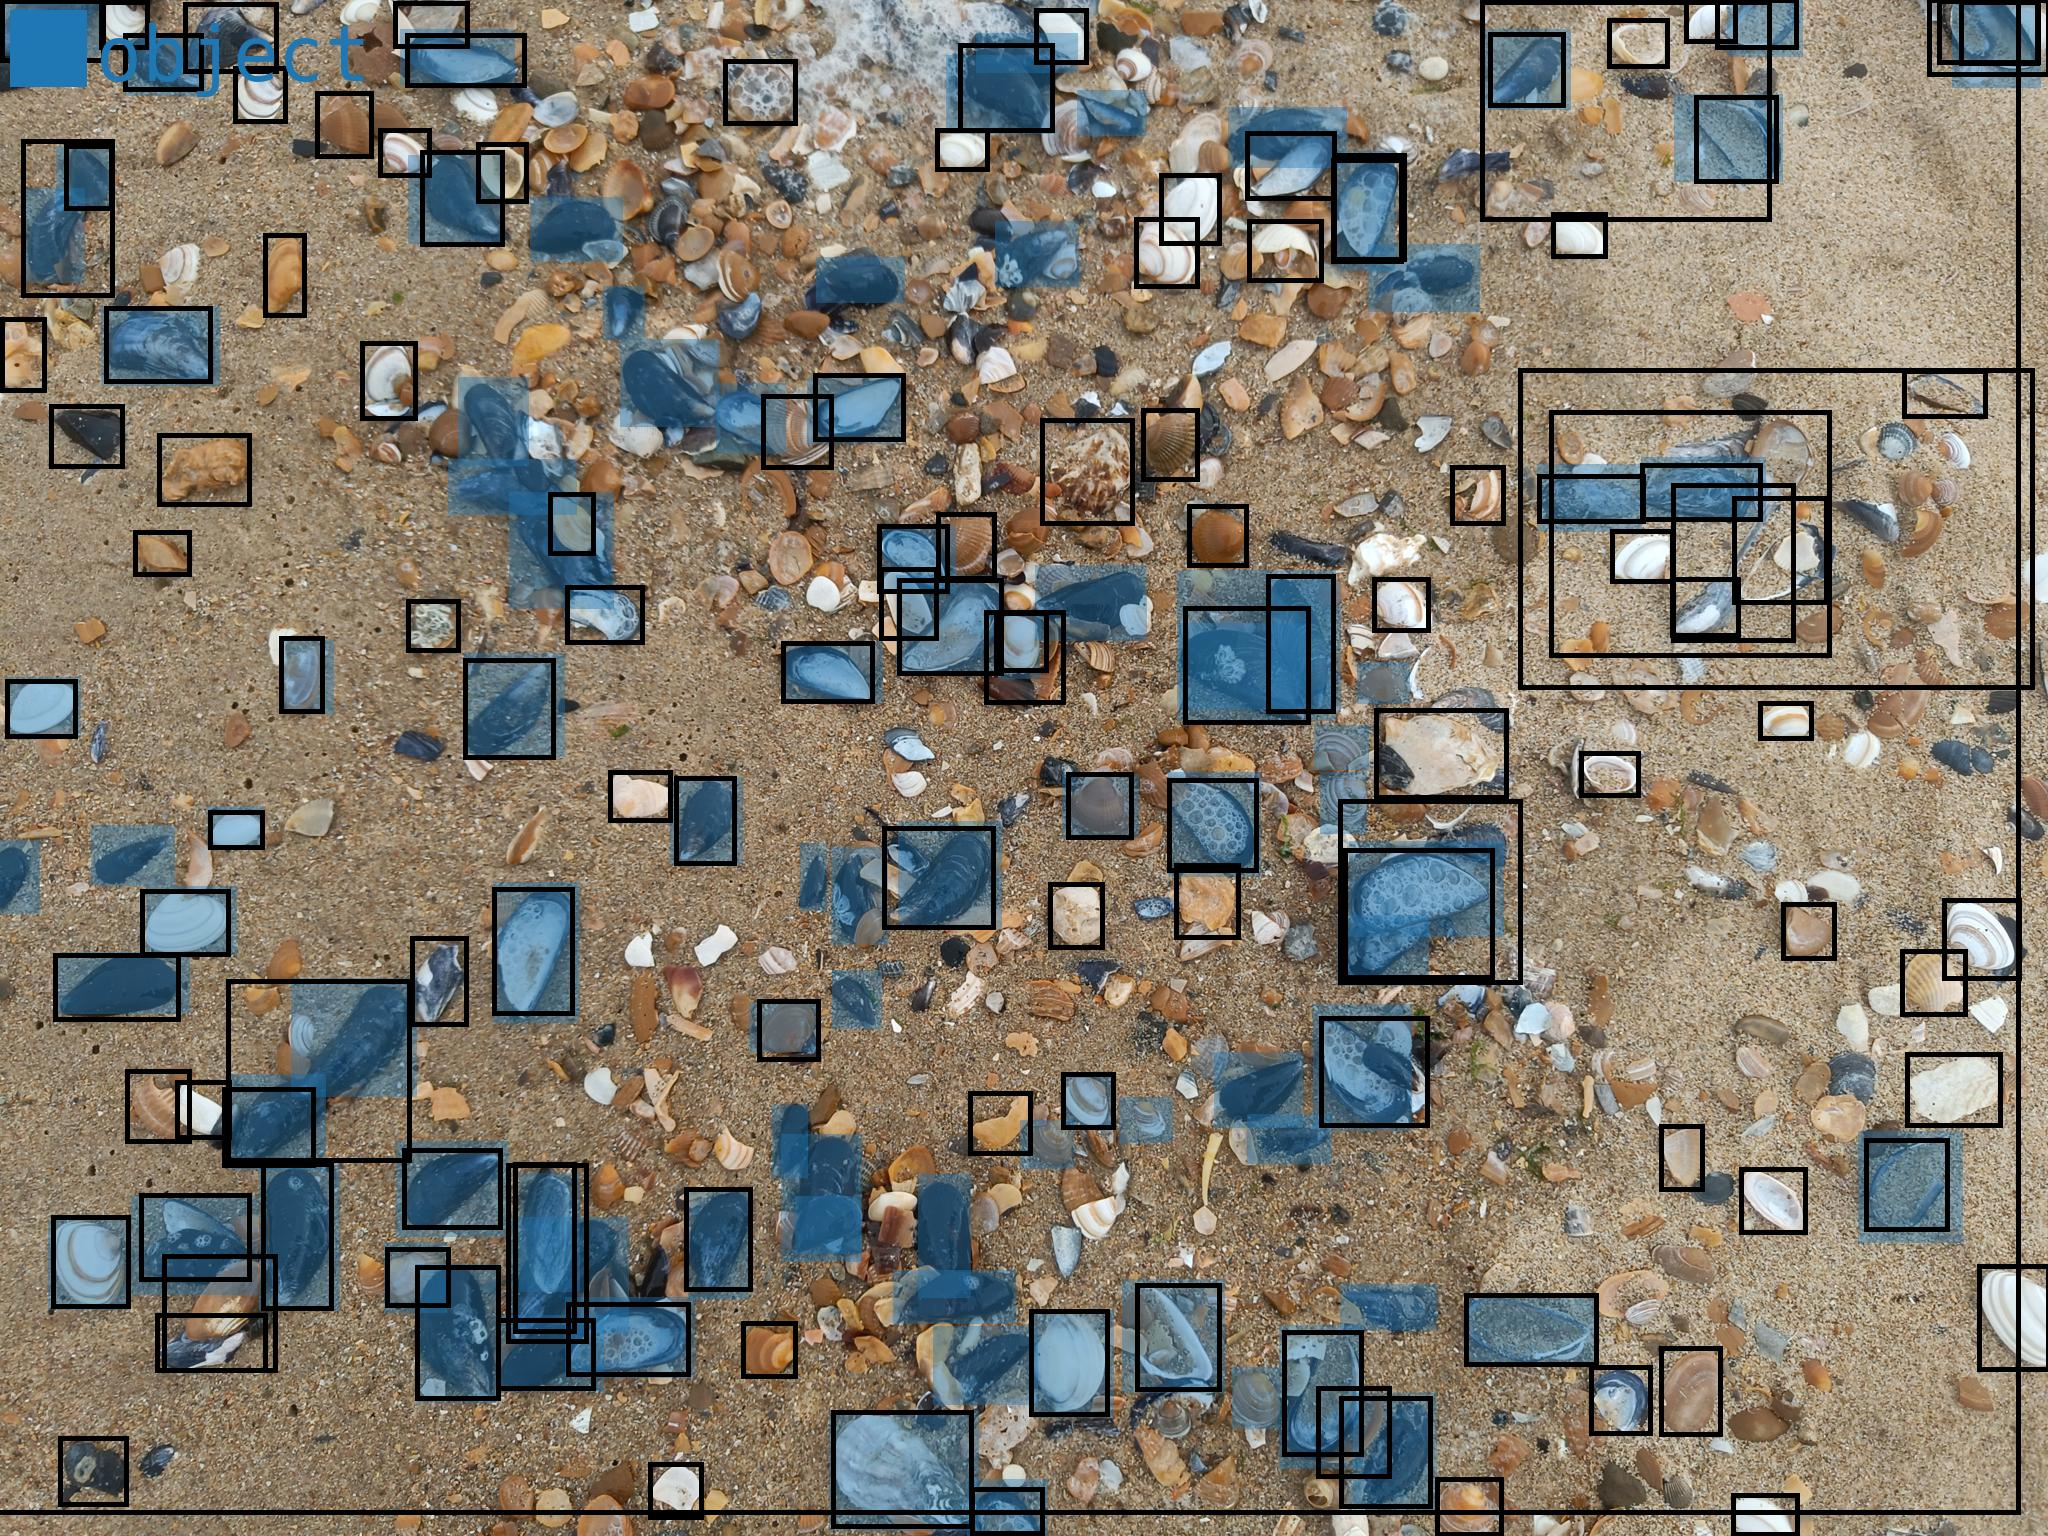
\includegraphics[width=0.3\textwidth]{chapter3/shell_examples/3.jpg}
    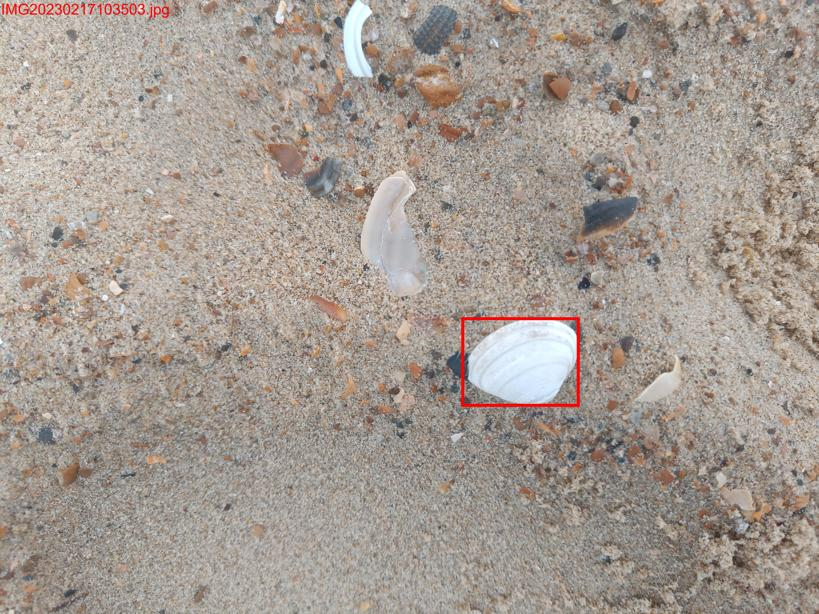
\includegraphics[width=0.3\textwidth]{chapter3/shell_examples/4.jpg} 
    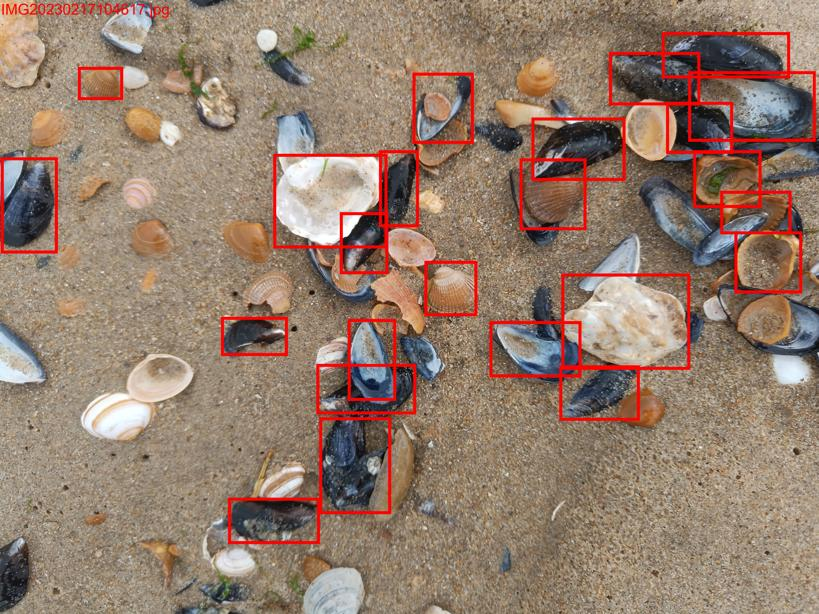
\includegraphics[width=0.3\textwidth]{chapter3/shell_examples/5.jpg} 
    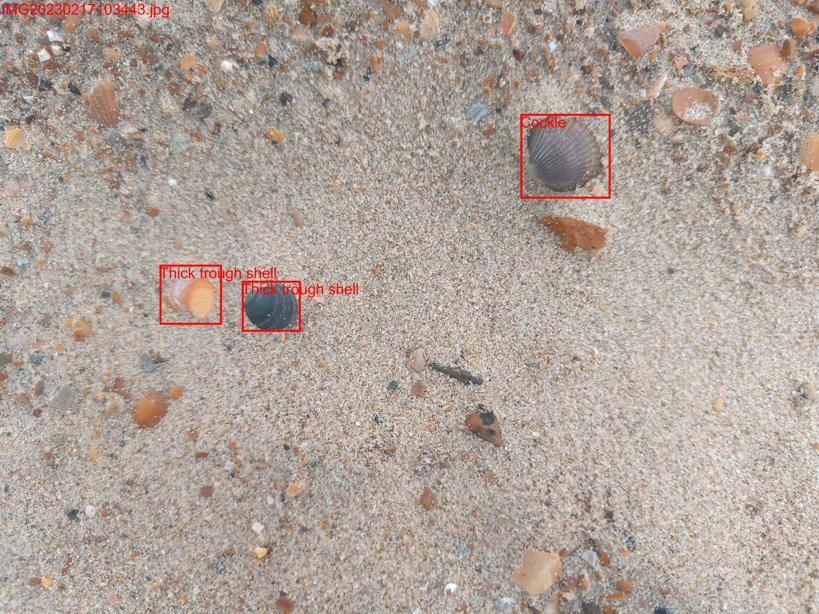
\includegraphics[width=0.3\textwidth]{chapter3/shell_examples/6.jpg}
    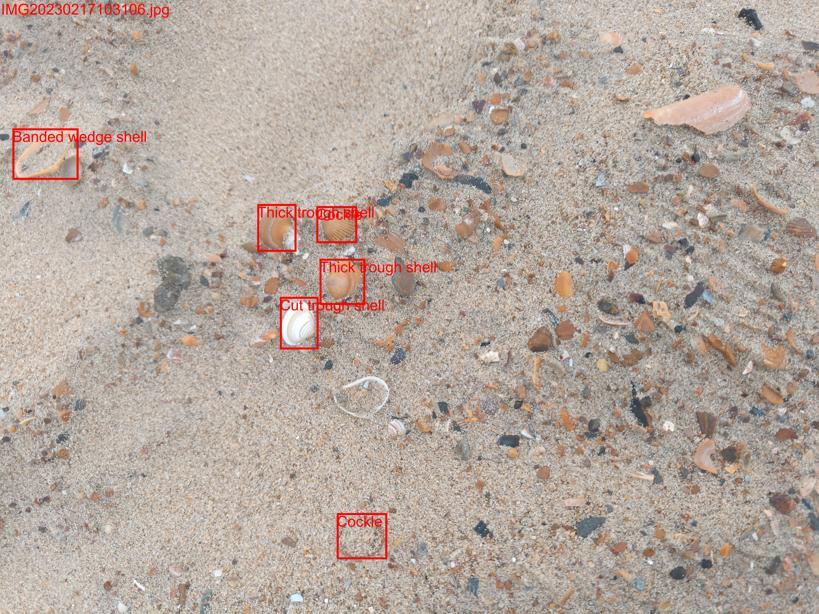
\includegraphics[width=0.3\textwidth]{chapter3/shell_examples/7.jpg}
    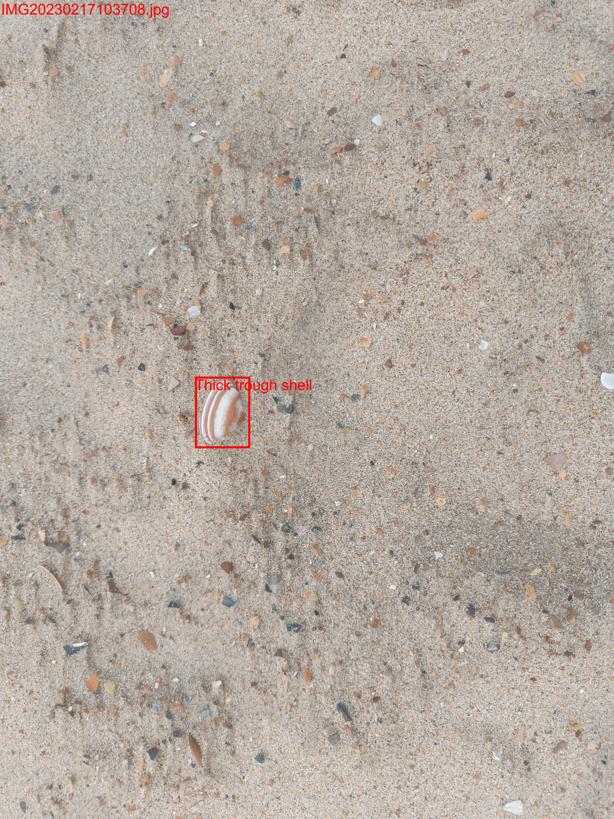
\includegraphics[width=0.3\textwidth]{chapter3/shell_examples/8.jpg}
    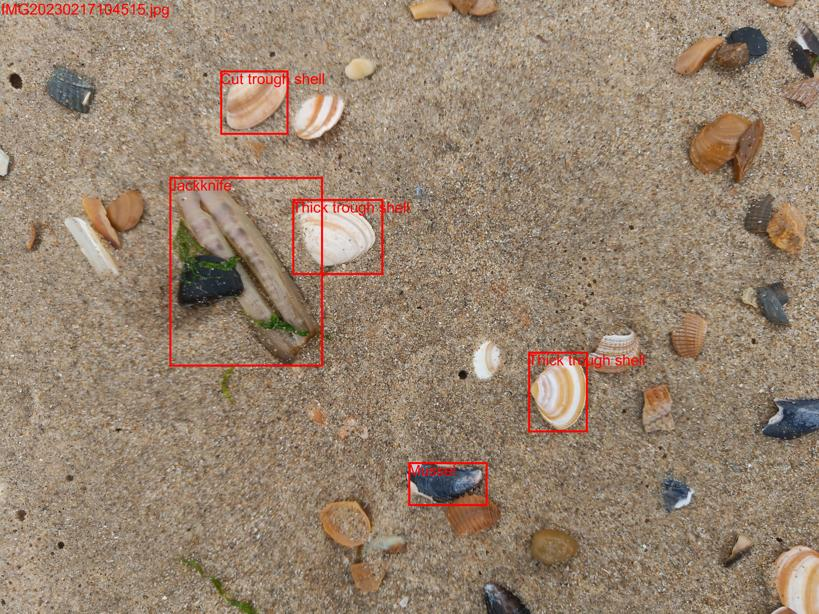
\includegraphics[width=0.3\textwidth]{chapter3/shell_examples/9.jpg}
    \caption{Examples of images in the shell dataset.}
    \label{tab:shell_examples}
\end{figure}